%%%%%%%%%%%%%%%%%%%%%%%%%%%%%%%%%%%%%%%%%%%%%%%%%%%%%%%%%%%%%%%%%%%%%%
% writeLaTeX Example: A quick guide to LaTeX
%
% Source: Dave Richeson (divisbyzero.com), Dickinson College
% 
% A one-size-fits-all LaTeX cheat sheet. Kept to two pages, so it 
% can be printed (double-sided) on one piece of paper
% 
% Feel free to distribute this example, but please keep the referral
% to divisbyzero.com
% 
%%%%%%%%%%%%%%%%%%%%%%%%%%%%%%%%%%%%%%%%%%%%%%%%%%%%%%%%%%%%%%%%%%%%%%
% How to use writeLaTeX: 
%
% You edit the source code here on the left, and the preview on the
% right shows you the result within a few seconds.
%
% Bookmark this page and share the URL with your co-authors. They can
% edit at the same time!
%
% You can upload figures, bibliographies, custom classes and
% styles using the files menu.
%
% If you're new to LaTeX, the wikibook is a great place to start:
% http://en.wikibooks.org/wiki/LaTeX
%
%%%%%%%%%%%%%%%%%%%%%%%%%%%%%%%%%%%%%%%%%%%%%%%%%%%%%%%%%%%%%%%%%%%%%%

\documentclass[10pt,landscape]{article}
\usepackage[T2A]{fontenc}
\usepackage[utf8]{inputenc}
\usepackage[russian]{babel}
\usepackage{graphicx}
\usepackage{amssymb,amsmath,amsthm,amsfonts}
\usepackage{multicol,multirow}
\usepackage{calc}
\usepackage{relsize}
% \usepackage{color,soul}
\usepackage{ifthen}
\usepackage[landscape]{geometry}
\usepackage[colorlinks=true,citecolor=blue,linkcolor=blue]{hyperref}


\ifthenelse{\lengthtest { \paperwidth = 11in}}
    { \geometry{top=.5in,left=.5in,right=.5in,bottom=.5in} }
	{\ifthenelse{ \lengthtest{ \paperwidth = 297mm}}
		{\geometry{top=1cm,left=1cm,right=1cm,bottom=1cm} }
		{\geometry{top=1cm,left=1cm,right=1cm,bottom=1cm} }
	}
\pagestyle{empty}
\makeatletter
\renewcommand{\section}{\@startsection{section}{1}{0mm}%
                                {-1ex plus -.5ex minus -.2ex}%
                                {0.5ex plus .2ex}%x
                                {\normalfont\large\bfseries}}
\renewcommand{\subsection}{\@startsection{subsection}{2}{0mm}%
                                {-1explus -.5ex minus -.2ex}%
                                {0.5ex plus .2ex}%
                                {\normalfont\normalsize\bfseries}}
\renewcommand{\subsubsection}{\@startsection{subsubsection}{3}{0mm}%
                                {-1ex plus -.5ex minus -.2ex}%
                                {1ex plus .2ex}%
                                {\normalfont\small\bfseries}}
\makeatother
\setcounter{secnumdepth}{0}
\setlength{\parindent}{0pt}
\setlength{\parskip}{0pt plus 0.5ex}
% -----------------------------------------------------------------------

\title{Quick Guide to LaTeX}

\begin{document}

\raggedright
\footnotesize

\begin{center}
     \Large{\textbf{Шпаргалка по математической статистике}} \\
\end{center}
\begin{multicols}{3}
\setlength{\premulticols}{1pt}
\setlength{\postmulticols}{1pt}
\setlength{\multicolsep}{1pt}
\setlength{\columnsep}{2pt}

\section{Схема математической статистики}
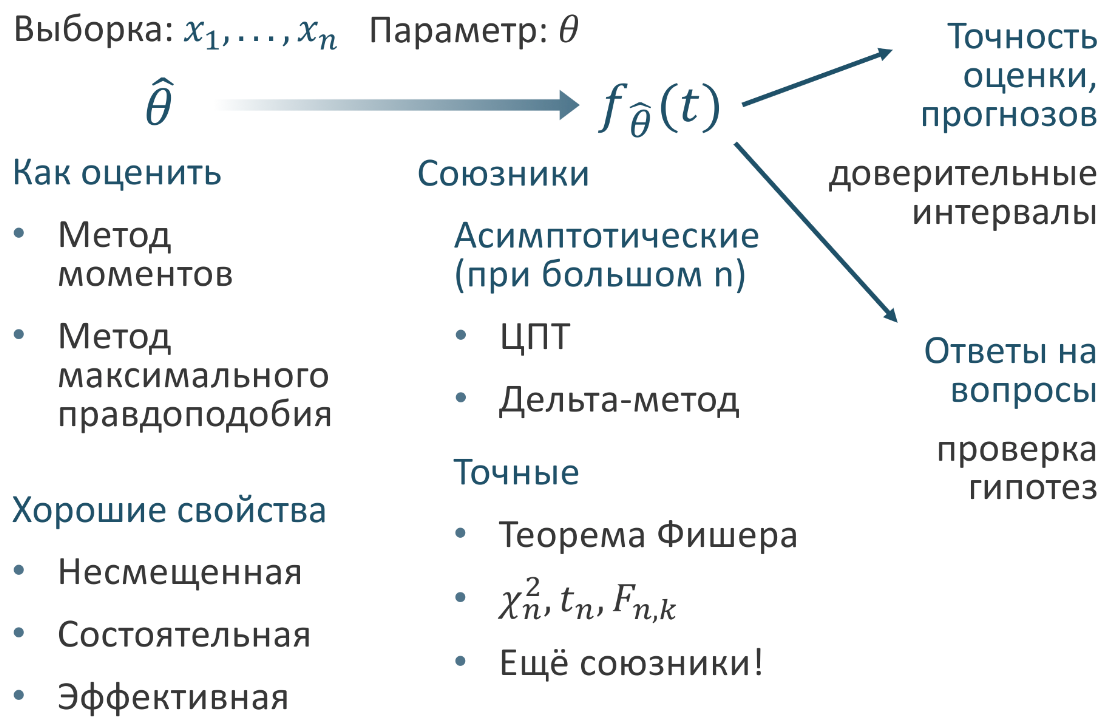
\includegraphics[width=0.3\textwidth]{Screenshot from 2021-07-20 12-12-42.png}

\section{Метод Моментов}
Чтобы использовать метод моментов, необходимо предположить две вещи:
\begin{enumerate}
    \item $X_1, ... , X_n \sim iid  \;$, \textit{Inependet and Identically Distributed random values}
    \item Предположить распределение из которого пришла выборка
\end{enumerate}
Момент $E(X_i^k)$ зависит от неизвестного параметра $\theta$: $E(X_i^k) = f(\theta)$

\textbf{Оценкой метода моментов} называется случайная величина: $\hat \theta_{MM} = f^{-1}(\overline{X^k})$\\
\textit{\textbf{Замечание:}} \textit{Нам позволяет так делать ЗБЧ, который говорит, что $\overline{X} = E(X)$}\\
\textit{\textbf{Замечание:}}\textit{Обычно хватает среднего первого порядка, но иногда нужно использовать более высокие порядки (например если среднее равно нулю)}

\section{Свойства оценок}
\subsection{Несмещенность}
Оценка называется \textbf{несмещённой}, если её математическое ожидание равно оцениваемому параметру: $E(\hat \theta) = \theta$

Смещение оценки это разница между её математическим ожиданием и её реальным значением: $bias(\hat \theta) = E(\hat \theta) - \theta$
 
\subsection{Состоятельность} 
Оценка называется \textbf{состоятельной}, если она сходится по вероятности к истинному значению параметра при $n \rightarrow \infty$ : $\hat \theta \xrightarrow{p} \theta$

\subsection{Асимптотическая несмещенность}
Оценка называется ассимтотически несмещенной, если её математическое ожидание сходится к оцениваемому параметру при $n \rightarrow \infty$, т.е: $E(\hat\theta) \xrightarrow[n\rightarrow\infty]{}\theta$

\subsection{Эффективность}
Обычно оценки сравнивают между собой с помощью квадратичной ошибки: $MSE = E(\hat\theta - \theta)^2$

\textit{Чем меньше, тем лучше}

\textbf{Статистик хочет получить:}
\begin{itemize}
    \item несмещенную оценку - хочет в среднем не ошибаться при фиксированном размере выборки
    \item состоятельную оценку - хочет при большом обьеме выборки быть близко к реальности
    \item оценку с маленькой средней квадратичной ошибкой
\end{itemize}
\subsection{Разложение на смещение и разброс}
$MSE = E(\hat \theta - E(\hat \theta))^2 + (E(\hat \theta)-\theta)^2 = Var(\hat \theta) + bias^2(\hat\theta)$
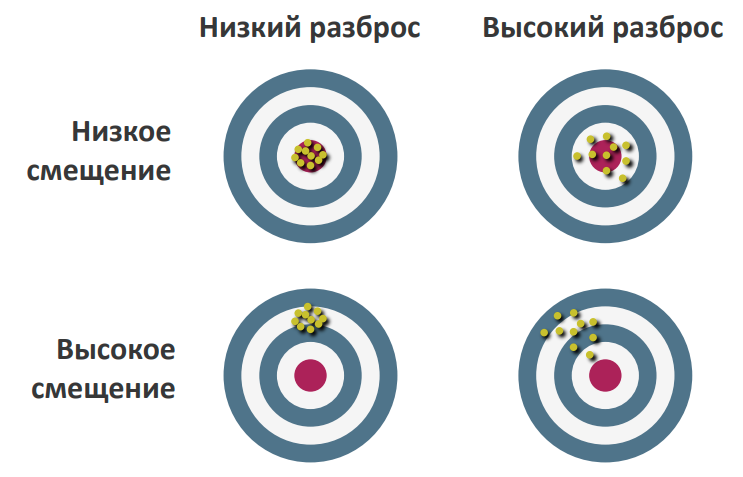
\includegraphics[width=0.3\textwidth]{Screenshot from 2021-07-20 12-29-32.png}

В классе всех возможных оценок наилучшей в смысле среднеквадратического подхода не существует, но можно зафиксировать смещение и найти оценку с наименьшей дисперсией(а.к.а. разбросом). Такая оценка называется эффективной в классе со смещением $bias(\hat\theta)$. Для функции потерь $MSE$ существует теоретическая нижняя граница, ее называют неравенством Рао-Фреше-Крамера.
\section{Неравенство Рао-Фреше-Крамера}
Если оценка параметра несмещена и выполнены условия регулярности:
\begin{itemize}
    \item Область определения случайной велечины не зависит от параметра $\theta$
    \item Можно брать производные от функции плотности
    \item Существует конечная $J(\theta) = E(\frac{\partial \ln f(x, \theta)}{\partial \theta})^2$
\end{itemize}
То верно: $Var(\hat \theta) \geq \frac{1}{n \cdot J(\theta)}$. 

Если оказалось, что  $Var(\hat \theta) = \frac{1}{n \cdot J(\theta)}$., то $\hat \theta$ - эффективная оценка для $\theta$

\textbf{\textit{Замечание:}} \textit{Если $\hat\theta$ - смещенная, то в числителе вместо 1 cтоит $(1+bias'\theta)^2$, а в остальном все аналогично}
\section{Доверительные интервалы}

Интервал $[\theta_L; \theta_U]$ называется \textbf{доверительным интервалом} для параметра \textbf{$\theta$}, с уровнем доверия \textbf{$1-\alpha$}, если при бесконечном повторении эксперимента в $100\cdot(1-\alpha)$ процентах случаев этот интервал будет накрывать значение параметра $\theta$

Величину $\alpha$ называют уровнем значимости



\textbf{Зачем нужны доверительные интервалы?}

\begin{itemize}

\item Точечная оценка делается по случайной выборке, а значит возникает неопределенность (т.к. выборка отличается от случая к случаю)

\item Нужно делать выводы в каком-то диапазоне

\item Доверительный интервал показывает, насколько мы уверены в точечной оценке

\end{itemize}

\textbf{\textit{Замечание:}} \textit{Обычно ищут наиболее короткий интервал, т.к. уже значит точнее}
\subsection{Асимптотический доверительный интервал для среднего}
\begin{itemize}
    \item ЦПТ позволяет построить интервал для любого среднего т.к. для ЦПТ не важно распределение величины
    \item Наблюдаем $X_1, ... , X_n$
    \item \textbf{Предполагаем:}$X_i$ независимо и одинаково распределены, число $n$ велико, \textbf{нет выбросов}
\end{itemize}
$\overline{x} \overset{asy}{\sim}  N(\mu, \frac{\sigma^2}{n}) \underset{\text{цент.}}{\Leftrightarrow} \overline{x} - \mu \overset{asy}{\sim} N(0,  \frac{\sigma^2}{n}) \underset{\text{норм.}}{\Leftrightarrow} \frac{\overline{x}-\mu}{\sqrt{\frac{\sigma^2}{n}}} \overset{asy}{\sim} N(0,  1)$

$p(\overline{x} - z_{1-\frac{\alpha}{2}} \frac{\hat \sigma}{\sqrt{n}} \leq \mu \leq \overline{x} + z_{1-\frac{\alpha}{2}} \frac{\hat \sigma}{\sqrt{n}}) = 1 - \alpha$

\textbf{\textit{или более просто:}} $\overline{x} \pm z_{1-\frac{\alpha}{2}} \frac{\hat \sigma}{\sqrt{n}}$
\subsection{Дельта-метод}
Если:\\
$X_1, ... , X_n \sim iid  \;$, $\; E(X_1) = \mu, Var(X_1) = \sigma^2$ и $g(t)$ - дифференцируемая функция, тогда: $g(\overline{x}) \sim N\big(g(\mu), \frac{\sigma^2}{n} \cdot g'(\mu)^2\big)$, \\\textbf{Тогда доверительный интервал:} $g(\overline{x}) \pm z_{1-\frac{\alpha}{2}} \frac{\hat \sigma}{\sqrt{n}}g'(\mu)$

\subsection{Асимптотический доверительный интервал для дисперсии}
$s^2 = \frac{n}{n-1}\hat{\sigma}^2 \Rightarrow s^2 \sim N\big(\sigma^2, \frac{\mu_4 - \sigma^4}{n}\big), \; \mu_4 = E[(X_i - \mu)^4]$
 Затем можно построить доверительный интервал, более подробно об интервалах для дисперсий смотри в разделе точных интервалов
\newpage

\subsection{Хи-квадрат распределение}
$X_1, ... , X_k \sim iid  \;  N(0, 1)$\\
$Y = X^2_1 + ... + X^2_k \sim \mathlarger{\chi}^2_k$\\
Характеристики:\\
$E(Y) = k, \; Var(Y) = 2k$\\
Плотность: $f(x) = \frac{1}{2^{\frac{k}{2}}\cdot \Gamma(\frac{k}{2})}\cdot x^{\frac{k}{2}-1}\cdot e^{-\frac{x}{2}}, \; x\geq0$


\subsection{Распределение Стьюдента}
$X_0\sim iid  \; N(0, 1)$, 
$Y  \sim X^2_k$\\
$Z = \frac{X_0}{\sqrt{Y/k}} \sim t(k)$\\
Характеристики:\\
$E(Z) = 0, \; Var(Z) = \frac{k}{k-2}, \; k > 2$\\
Плотность: $f(x) = \frac{\Gamma(\frac{k+1}{2})}{\sqrt{\pi k} \cdot \frac{k}{2}} \cdot (1 + \frac{x^2}{k})^{-\frac{k+1}{2}}$

\subsection{Распределение Фишера}
$X \sim X^2_k$, 
$Y  \sim X^2_k$\\
$Z = \frac{\sqrt{X/k}}{\sqrt{Y/m}} \sim F(k,m)$\\
Характеристики:\\
$E(Z) = \frac{m}{m-2}, \; m > 2, \; Var(Z) = \frac{2m^2(k+m-2)}{k(m-2)^2(m-4)}, \; m > 4$\\
Плотность: *тут очень большая формула*

\subsection{Теорема Фишера}
Пусть $X_1, ... , X_k \sim iid  \; N(0, 1)$, тогда
\begin{enumerate}
    \item Выборочное среднее $\overline{x}$ и дисперсия $s^2$ независимы
    \item $\frac{(n-1)\cdot s^2}{\sigma^2}$ имеет $\mathlarger{\chi}^2 $ - распределение с $n-1$ степенью свободы т.е. $\frac{(n-1)\cdot s^2}{\sigma^2} \sim \mathlarger{\chi}^2_{n-1}$
\end{enumerate}


\section{Точные доверительные интервалы для нормальных выборок}
\textbf{Обязательное условие:} $X_1, ... , X_n \sim iid  \;  N(\mu, \sigma^2)$ 

\subsection{Точный доверительный интервал для среднего}
\begin{itemize}
    \item \textbf{Дисперсия известна}
    $\sigma^2$ - известна и $\hat \mu = \overline{x}=\frac{X_1 + ... + X_n}{n} \sim N(\mu, \frac{\sigma^2}{n})$\\
   \textbf{ Тогда доверительный интервал:}
   $p(\overline{x} - z_{1-\frac{\alpha}{2}}\frac{\sigma}{\sqrt{n}} \leq \mu \leq \overline{x} + z_{1-\frac{\alpha}{2}}\frac{\sigma}{\sqrt{n}}) = 1 - \alpha$ или проще: $\overline{x} \pm z_{1-\frac{\alpha}{2}}\frac{\sigma}{\sqrt{n}}$
   \item \textbf{Дисперсия не известна}
    $\sigma^2$ - не известна и $\hat \mu = \overline{x}\sim N(\mu, \frac{\sigma^2}{n})$\\
    $\frac{\overline{x}-\mu}{\sqrt{\frac{s^2}{n}}} \sim t(n-1)$\\
    \textbf{ Тогда доверительный интервал:}
    $p(\overline{x} - t_{1-\frac{\alpha}{2}}\frac{s}{\sqrt{n}} \leq \mu \leq \overline{x} +  t_{1-\frac{\alpha}{2}}\frac{s}{\sqrt{n}}) = 1 - \alpha$ или проще: $\overline{x} \pm t_{1-\frac{\alpha}{2}}\frac{s}{\sqrt{n}}$
\end{itemize}
\subsection{Точный vs Асимптотический}

\includegraphics[width=0.3\textwidth]{Screenshot from 2021-07-23 12-53-12.png}
\subsection{Точные доверительные интервалы для разности средних}
\textbf{Дисперсии неизвестны (асимптотика)}\\
$\overline{x} - \overline{y} \pm z_{1-\frac{\alpha}{2}} \cdot \sqrt{\frac{s^2_x}{n_x}+\frac{s^2_y}{n_y}}$\\
\textbf{Дисперсии известны (точный)}\\
$\overline{x} - \overline{y} \pm z_{1-\frac{\alpha}{2}} \cdot \sqrt{\frac{\sigma^2_x}{n_x}+\frac{\sigma^2_y}{n_y}}$\\
\textbf{Дисперсии неизвестны, но равны (точный)}\\
$\overline{x} - \overline{y} \pm t(n_x+n_ - 2)_{1-\frac{\alpha}{2}} \cdot \sqrt{\frac{s^2}{n_x}+\frac{s^2}{n_y}}$\\
\textbf{Дисперсии неизвестны и не равны (примерный)}\\
$\overline{x} - \overline{y} \pm t(v)_{1-\frac{\alpha}{2}} \cdot \sqrt{\frac{s^2_x}{n_x}+\frac{s^2_y}{n_y}}$\\
где $v$ - приближенное распределение Уэлча
\subsection{Точные доверительные интервалы для дисперсии}
\begin{itemize}
    \item Мат. ожидание известно
    $p(\frac{n\cdot s^2}{\chi^2_n(1-\frac{\alpha}{2})} \leq \sigma^2 \leq \frac{n\cdot s^2}{\chi^2_n(\frac{\alpha}{2})}) = 1 - \alpha$
    \item Мат. ожидание НЕизвестно
    $p(\frac{(n-1)\cdot s^2}{\chi^2_{(n-1)}(1-\frac{\alpha}{2})} \leq \sigma^2 \leq \frac{(n-1)\cdot s^2}{\chi^2_{(n-1)}(\frac{\alpha}{2})}) = 1 - \alpha$
\end{itemize}
\subsection{Точный доверительный интервал для отношения дисперсий независимых выборок}
$\frac{s^2_m}{s^2_n}F_{n-1,m-1}(\frac{\alpha}{2})\leq \frac{\sigma^2_m}{\sigma^2_n} \leq \frac{s^2_m}{s^2_n}F_{n-1,m-1}(1-\frac{\alpha}{2})$
\section{Проверка гипотез}
Гипотеза - утверждение, которое возникло в нашей голове и которое мы собираемся проверить по данным.
\subsection{Процедура проверки гипотез}
\begin{enumerate}
    \item Фиксируем уровень значимости $\alpha$ (вероятность зря отвергнуть нулевую гипотезу)
    \item Формируем нулевую $H_0$ и альтернативную $H_a$ гипотезы
    \item Выбираем союзника для проверки гипотезы 
    \item Находим наблюдаемое значение
    \item Находим критическое значение с помощью союзника
    \item Сравниваем наблюдаемое значение с критическим и делаем выводы
\end{enumerate}
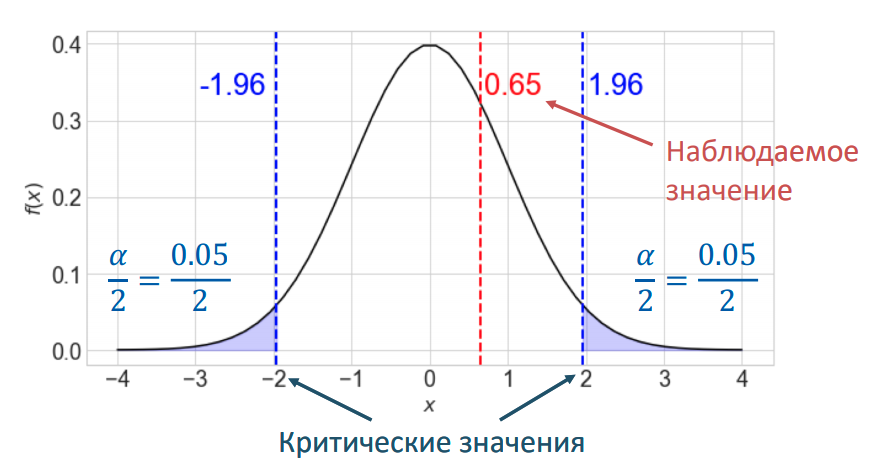
\includegraphics[width=0.32\textwidth]{Screenshot from 2021-09-03 10-49-36.png}
\subsection{p-значение}
p-значение - это достигаемый уровень значимости
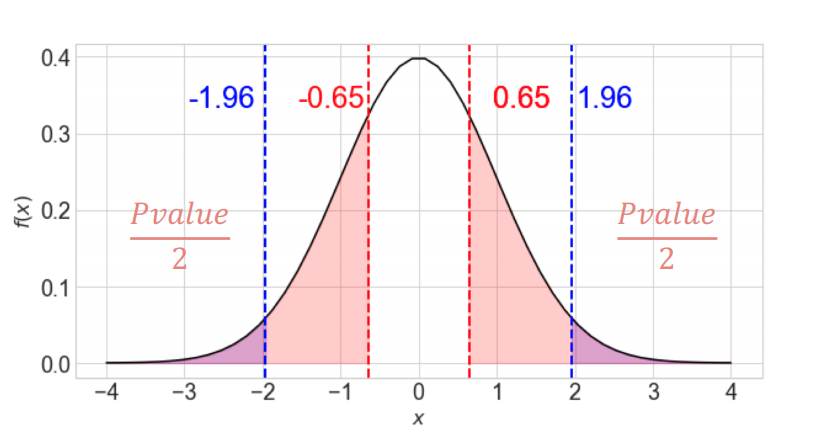
\includegraphics[width=0.32\textwidth]{Screenshot from 2021-09-03 11-05-29.png}
\begin{itemize}
    \item если $p\_value > \alpha$, то наблюдаемое значение попало в область между критическими, а значит гипотеза  \textbf{не отвергается}
    \item если $p\_value < \alpha$, то наблюдаемое значение не попало в область между критическими, а значит гипотеза \textbf{отвергается}
\end{itemize}
\textbf{Вопрос:} \textit{Какой уровень значимости надо брать, чтобы гипотеза впервые отверглась?}\\
\textbf{Ответ:} \textit{равный p-значению}

\subsection{Ошибки 1-ого и 2-ого рода}
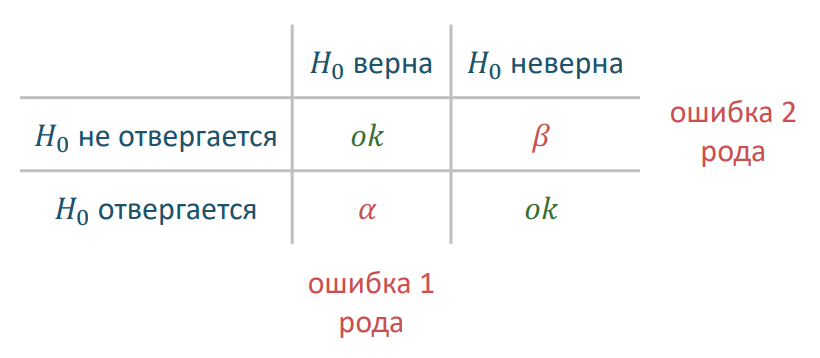
\includegraphics[width=0.32\textwidth]{Screenshot from 2021-09-03 11-16-31.png}
$\alpha = P(H_0 \;\text{ отвергнута}\; |\; H_0 \; \text{верна})$\\
$\beta = P(H_0 \;\text{не отвергнута}\; |\; H_0 \;\text{не верна})$\\
Величину $1 - \beta$ называют \textbf{мощностью} критерия
\textit{\textbf{Замечание:} При уменьшении ошибки первого рода всегда возрастает ошибка второго рода}



\newpage

\section{Параметрические критерии}
Включают в себя расчёт параметров конкретного распределения (т.е. предполагаем, что данные пришли из определенного распределения)
\subsection{Критерии о долях}
\textbf{Z-критерий для доли}\\
$X_1, ... , X_N \sim iid Bern(p)$\\
$H_0 : p = p_0$\\
$H_a : p \neq p_0$\\
ЦПТ: 
$\hat{p} \underset{H_0}{\overset{asy}{\sim}} N\Big(p_0, \frac{p_0(1-p_0)}{n}\Big)$\\
Критерий для проверки: $z = \frac{\hat{p}-p_0}{\sqrt{\frac{p_0(1-p_0)}{n}}}\underset{H_0}{\overset{asy}{\sim}} N(0,1) $\\
\textbf{Z-критерий для разности независимых долей}\\
$X_1, ... , X_N \sim iid Bern(p_x)$\\
$Y_1, ... , Y_N \sim iid Bern(p_y)$\\
Выборки независимые\\
$H_0: p_x = p_y$, $H_a: p_x \neq p_y$\\
$z = \frac{\hat{p_x}-\hat{p_y}}{\sqrt{P(1-P) \cdot (\frac{1}{n_x} + \frac{1}{n_y})}}\underset{H_0}{\overset{asy}{\sim}} N(0,1), \; P = \frac{m_x + m_y}{n_x + n_y}$, где $m_i$ - число 1 в выборке\\

\textbf{Z-критерий для разности зависимых долей}\\
$X_1, ... , X_N \sim iid Bern(p_x)$\\
$Y_1, ... , Y_N \sim iid Bern(p_y)$\\
Выборки независимые\\
$H_0: p_x = p_y$, $H_a: p_x \neq p_y$\\
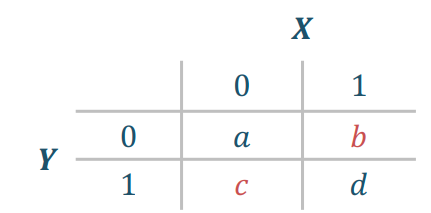
\includegraphics[width=0.25\textwidth]{Screenshot from 2021-09-03 12-13-14.png}
$z = \frac{c - b}{\sqrt{ c + b  - \frac{(c-b)^2}{n}}}\underset{H_0}{\overset{asy}{\sim}} N(0,1)$\\

\subsection{Критерии о средних}
\textbf{Z-критерий для средних}\\
$X_1, ... , X_N \sim iid (\mu, \sigma^2)$\\
$H_0 : \mu = \mu_0$\\
$H_a : \mu \neq \mu_0$\\
ЦПТ: 
$\overline{x} \underset{H_0}{\overset{asy}{\sim}} N\Big(\mu_0, \frac{\hat{\sigma^2}}{n}\Big)$\\
Критерий для проверки: $z = \frac{\overline{\mu}-\mu_0}{\sqrt{\frac{\hat{\sigma^2}}{n}}}\underset{H_0}{\overset{asy}{\sim}} N(0,1) $\\
\textit{\textbf{Замечание:} Данный критерий может быть использован для любых распределений, а вот следующий только для нормального}\\ 
\textbf{t-критерий для средних}\\
$X_1, ... , X_N \sim iid N(\mu, \sigma^2)$\\
$H_0 : \mu = \mu_0$\\
$H_a : \mu \neq \mu_0$\\
$\sigma^2$ - известна\\
ЦПТ: 
$\overline{x} \underset{H_0}{\sim} N\Big(\mu_0, \frac{\sigma^2}{n}\Big)$\\
Критерий для проверки: $z = \frac{\overline{\mu}-\mu_0}{\sqrt{\frac{\sigma^2}{n}}}\underset{H_0}{\sim} N(0,1) $\\


$\sigma^2$ - НЕ известна\\
ЦПТ: 
$\overline{x} \underset{H_0}{\sim} N\Big(\mu_0, \frac{\sigma^2}{n}\Big)$\\
Критерий для проверки: $z = \frac{\overline{\mu}-\mu_0}{\sqrt{\frac{s^2}{n}}}\underset{H_0}{\sim} t(n-1) $\\

\textbf{Z-критерий для разности средних}\\
$X_1, ... , X_N \sim iid (\mu_1, \sigma^2_1)$\\
$Y_1, ... , Y_N \sim iid (\mu_2, \sigma^2_2)$\\
Выборки независимые \\
$H_0 : \mu_1 = \mu_2$\\
$H_a : \mu_1 \neq \mu_2$\\

ЦПТ: 
$\overline{X_1} - \overline{X_2} \underset{H_0}{\overset{asy}{\sim}} N\Big(0, \frac{s_1^2}{n}+\frac{s_2^2}{m}\Big)$\\
Критерий для проверки: $z = \frac{\overline{X_1} - \overline{X_2}}{\sqrt{\frac{s_1^2}{n}+\frac{s_2^2}{m}}}\underset{H_0}{\overset{asy}{\sim}} N(0,1) $\\
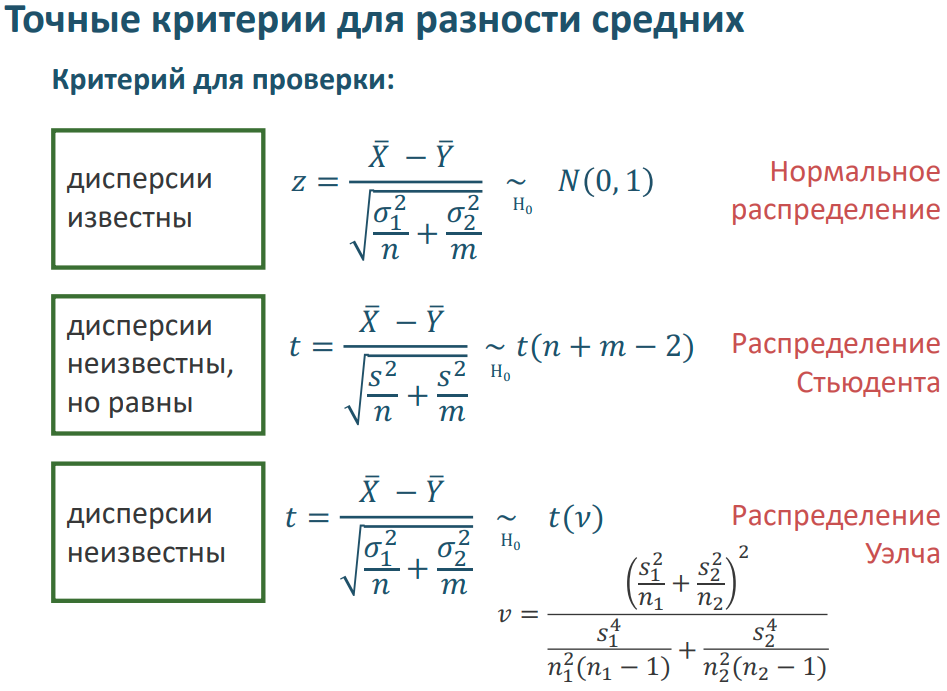
\includegraphics[width=0.3\textwidth]{Screenshot from 2021-09-04 10-53-10.png}
\\
\subsection{Критерии о дисперсиях}
$\chi^2$ \textbf{ - критерий для дисперсии}\\
$X_1, ... , X_N \sim iid N(\mu, \sigma^2)$\\
$\mu$ - известно\\
$H_0: \sigma^2 = \sigma^2_0$\\
$H_a: \sigma^2 > \sigma^2_0$\\
Критерий для проверки:\\
$\frac{n * s^2}{\sigma^2_0} = \sum\limits_{i=1}^{n} \frac{(X_i - \mu)^2}{\sigma^2_0} \underset{H_0}{\sim}\chi^2_n$
\begin{itemize}
    \item Высокая дисперсия связана с риском и нестабильностью
    \item Мы хотим знать, принимает ли дисперсия своё значение ниже $\sigma_0^2$
    \item Из-за этого в качестве альтернативы обычно используют правостороннюю
\end{itemize}
$\mu$ - НE известно\\
$H_0: \sigma^2 = \sigma^2_0$\\
$H_a: \sigma^2 > \sigma^2_0$\\
Критерий для проверки:\\
$\frac{(n-1) * s^2}{\sigma^2_0} = \sum\limits_{i=1}^{n} \frac{(X_i - \mu)^2}{\sigma^2_0} \underset{H_0}{\sim}\chi^2_{(n-1)}$\\
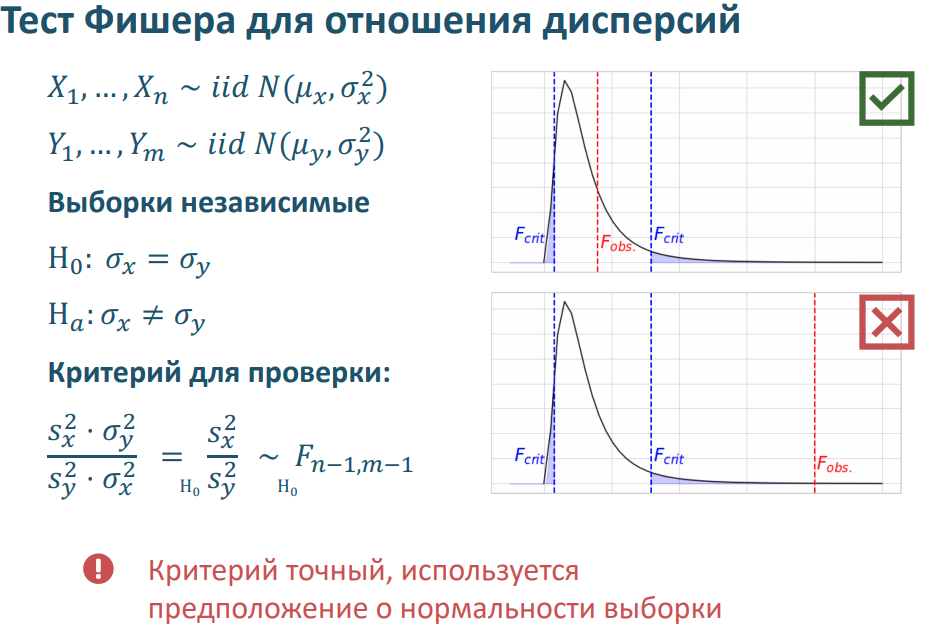
\includegraphics[width=0.3\textwidth]{Screenshot from 2021-09-04 11-12-01.png}

\section{Непараметрические критерии}
Такие критерии помогают не зацикливаться на том из какого распределения пришла выборка\\
\subsection{Критерий знаков}
Идея: Превратить выборку в нули и единицы => можем использовать биномиальное распределение\\
Минусы: Теряем часть информации зашитой в выборку\\
\textbf{Пример:} Критерий знаков(одновыборочный)
$X_1, ..., X_n \sim iid$\\
$H_0: Median(X) = m_0$\\
$H_a: Median(X) \neq m_0$\\
Критерий для проверки:\\
$T = \sum\limits_{i=1}^n[X_i > m_0] \sim Bin(0.5, n)$\\

\textbf{Пример:} Критерий знаков(двухвыборочный)
$X_1, ..., X_n \sim iid$\
$Y_1, ..., Y_n \sim iid$\\
Выборки связанные\\
$H_0: P(X>Y) = 0.5$\\
$H_a: P(X>Y) \neq 0.5$\\
Критерий для проверки:\\
$T = \sum\limits_{i=1}^n[X_i > Y_i] \sim Bin(0.5, n)$\\
\newpage
\subsection{Ранговые критерии}
$x_1, x_2, ... , x_n$ - выборка \\
$x_{(1)} \leq x_{(3)} \leq ... \leq x_{(n)}$ - упорядочим по возрастанию\\

Правила выставления ранга:
\begin{enumerate}
    \item Порядковый номер наблюдения - ранг
    \item Если встречаются несколько одинаковых значений, им присваивается одинаковое значение ранга, равное среднему арифметическому их порядковых номеров
\end{enumerate}
\textbf{Критерий Уилкоксона (одновыборочный)}\\
$X_1, ... , X_n \sim iid$\\
$F_X(x)$ - симметрична относительно медианы\\
$H_0: Median(X) = m_0$\\
$H_a: Median(X) \neq m_0$\\
Критерий для проверки:\\
$W = \sum\limits_{i=1}^n rank(|X_i - m_0|) * sign(X_i-m_0)$ - табличное распределение\\

\textbf{Критерий Уилкоксона (двухвыборочный)}\\
Предполагаем, что распределения одинаковые, хотим проверить сдвинутые ли они
$X_1, ... , X_n \sim iid$\\
$Y_1, ... , Y_n \sim iid$\\
Выборки связанные\\
$H_0: Median(X - Y) = 0$\\
$H_a: Median(X - Y) \neq 0$\\
Критерий для проверки:\\
$W = \sum\limits_{i=1}^n rank(|X_i - Y_i|) * sign(X_i-Y_i)$ - табличное распределение\\
\textbf{Критерий Манна-Уитни(двухвыборочный)}\\
$X_1, ... , X_{n_x} \sim iid$\\
$Y_1, ... , Y_{n_y} \sim iid$\\
Выборки независимые\\
$n_x \leq n_y$\\
$H_0: f_X(x) =  f_Y(y) $\\
$H_a: f_X(x) =  f_Y(y + m), m \neq 0$\\
Объединим обе выборки в одну общую и посчитаем для всех чисел ранги\\
Критерий для проверки:\\
$ W = \sum\limits_{i=1}^{n_x} rank(X_i)$ - табличное распределение
\section{Бутстрап}
\textbf{Идея метода:} имеющаяся выборка - это единственная информация об истинном распределении данных
\subsection{Доверительный интервал Эфрона}
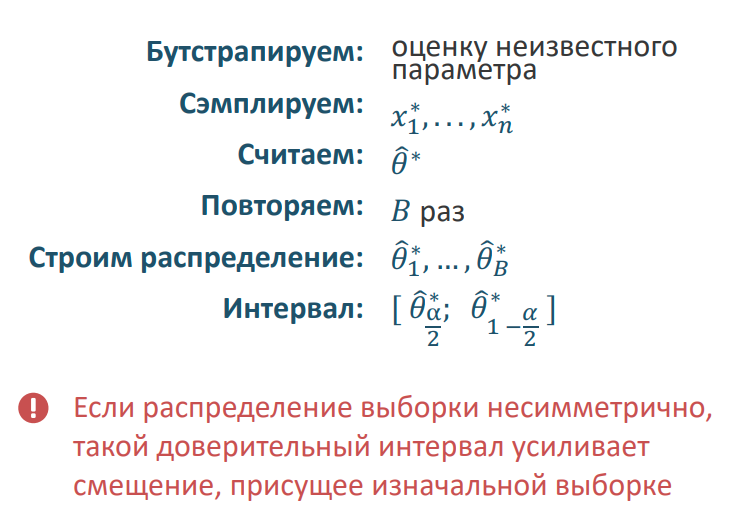
\includegraphics[width=0.3\textwidth]{Screenshot from 2021-09-08 11-06-02.png}
\subsection{Доверительный интервал Холла}
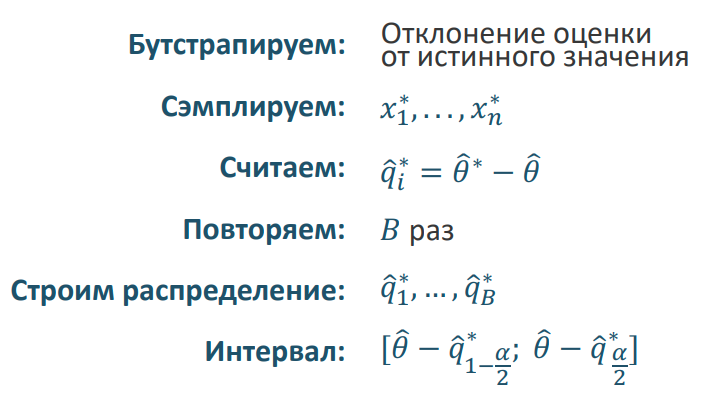
\includegraphics[width=0.3\textwidth]{Screenshot from 2021-09-08 11-46-04.png}
\subsection{t-процентильный доверительный интервал}
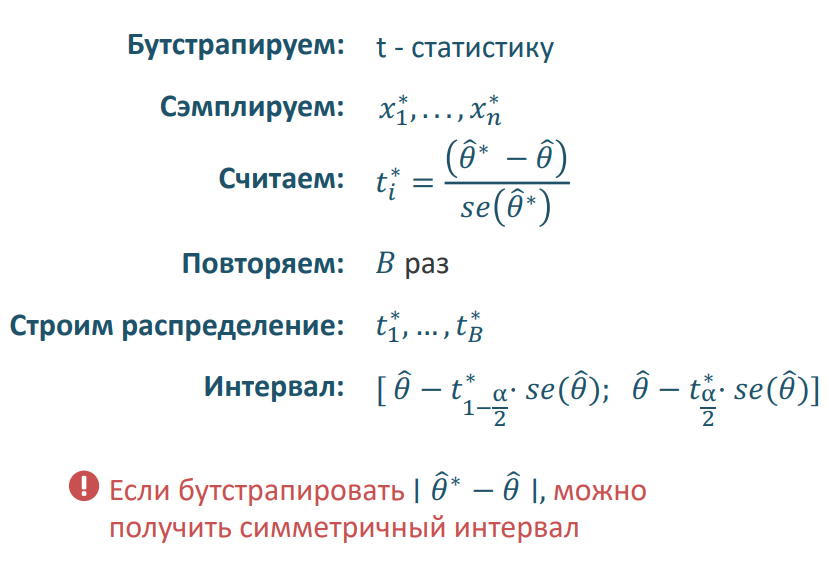
\includegraphics[width=0.3\textwidth]{Screenshot from 2021-09-08 11-47-25.png}
\subsection{Проблемы бутстрапа}
\begin{itemize}
    \item Чтобы бутстрап сработал, выборка должна быть
репрезентативной
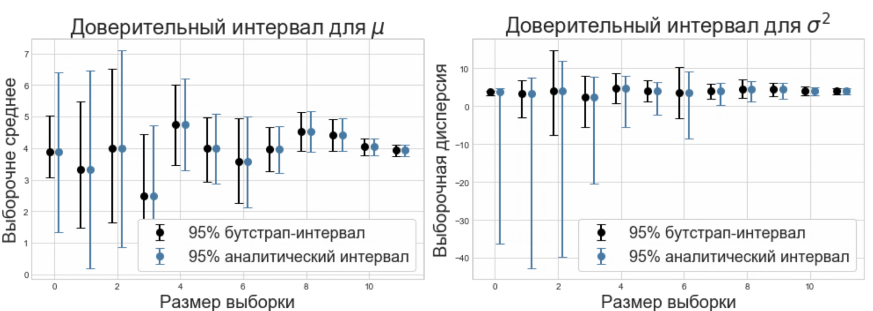
\includegraphics[width=0.3\textwidth]{Screenshot from 2021-09-08 11-50-39.png}
\item Если исходная выборка маленькая, бутстраповский
доверительный интервал будет уже аналитического,
так как в выборке недостаточно “неопределенности”
\item Если в данных есть структура (регрессия, временные
ряды), бутстрап нужно устроить так, чтобы учитывать
её $\Rightarrow$ разные виды бутстрапа
\item Бутстрап ненадёжно работает в хвостах распределения
из-за маленького числа наблюдений: мы можем хорошо
оценить медиану, но не 99\% квантиль
\item Если у распределения тяжёлые хвосты, бутстрап может
работать некорректно и в средиземье
\end{itemize}
\subsection{Проверка гипотез при прмощи бутсрапа}
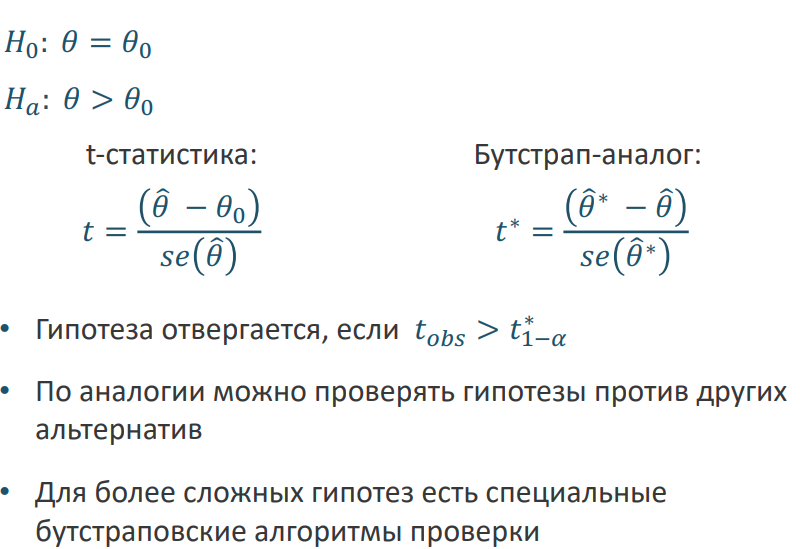
\includegraphics[width=0.3\textwidth]{Screenshot from 2021-09-08 12-00-54.png}
\newpage
\section{Критерии согласия}
\subsection{Эмпирическая функция распределение}
\textbf{Функция распределения} – функция, которая определяет
вероятность события $X\leq x$, то есть $F(x) = P(X \leq x)$ \\

\textbf{Эмпирическая функция распределения} – функция, которая
определяет для каждого $x$ частоту события $X\leq x$, то есть $\hat{F}_n(x) = \hat{P}(X \leq x) = \frac{1}{n}\sum\limits_{i=1}^n [X_i \leq x]$, [] - индикатор

\textbf{Свойства эмперической функции распределения}
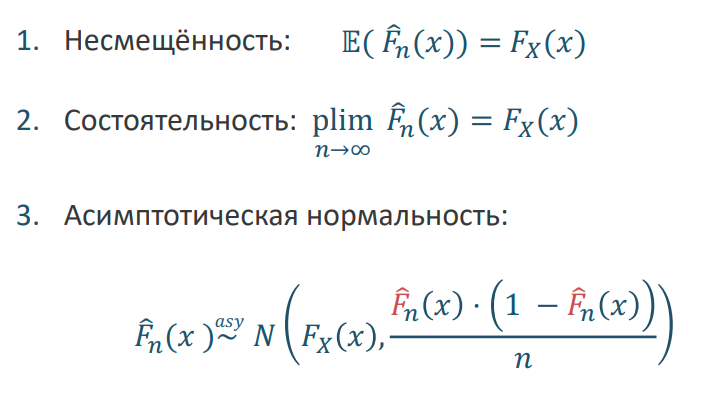
\includegraphics[width=0.3\textwidth]{Screenshot from 2021-09-10 11-13-49.png}
\subsection{Критерий Колмогорова}
Используется для проверки гипотез о непрерывных распределениях
\begin{itemize}
    \item Критерии согласия - критерий о виде неизвестного закона распределения: 
    $H_0: X \sim F_x(x)$, 
    $H_a:$ гипотеза $H_0$ неверна
    \item Распределение случайной величины описывается её функцией распределения:
    $H_0: F_x(x) = F_0(x)$, 
    $H_a: F_x(x) \neq F_0(x)$
\end{itemize}
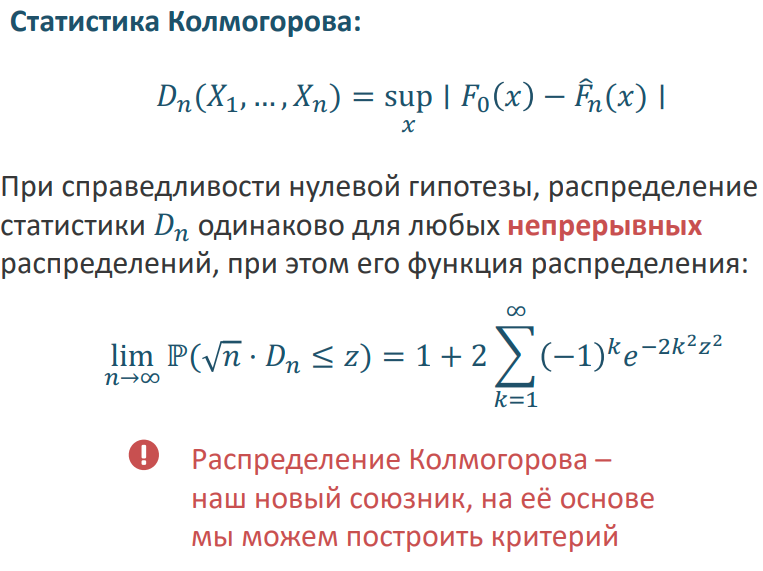
\includegraphics[width=0.3\textwidth]{Screenshot from 2021-09-10 11-41-04.png}
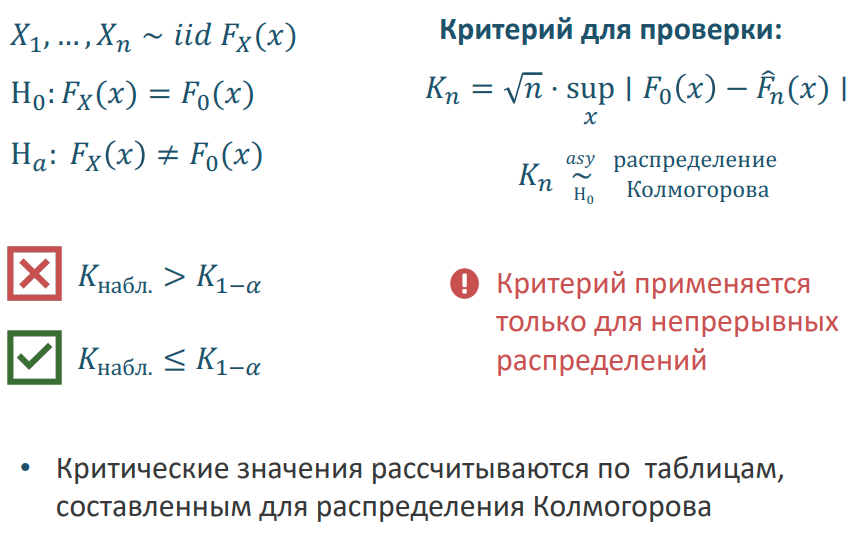
\includegraphics[width=0.3\textwidth]{Screenshot from 2021-09-10 11-42-22.png}
\textit{\textbf{Замечание:}} \textit{Для проверки гипотезы об однородности двух выборок, можно также пользоваться этой идеей, просто считать расстояние между двумя эмперическими функциями}\\
\textit{\textbf{Замечание:}}
\textit{
\begin{itemize}
    \item Чтобы проверять гипотезы о распределениях,
нужно научиться считать между ними расстояния
    \item Критерий Колмогорова ищет расстояние как супремум
и позволяет проверять гипотезы о распределении
и однородности выборок
    \item Критерии Крамера-Мизеса и Андерсона-Дарлинга
помогают специфицировать критерий либо для
”средиземья” либо для ”крайнеземья” (хвостов)
    \item Эти критерии работают только для непрерывных
распределений 
    \item Неизвестные параметры распределения фиксируются
в нулевой гипотезе
    \item Если мы оцениваем параметры по выборке,
распределения Колмогорова не будет одинаковым
для всех распределений
    \item Для различных распределений можно строить уточнения
теста Колмогорова
\end{itemize}
}
\subsection{Критерий Пирсона}
Используется для проверки гипотез о дискретных распределениях
\begin{itemize}
    \item Выборка $X_1, ..., X_n$ из дискретного распределения
    \item Предполагаем, что случайная величина принимает $s$
значений с какими-то вероятностями
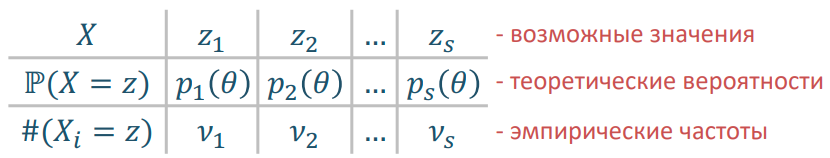
\includegraphics[width=0.3\textwidth]{Screenshot from 2021-09-10 11-53-16.png}
    \item Нужно сравнить все эмпирические частоты
с теоретическими
    $\hat{\theta}$ - состоятельная
оценка параметров
распределения, $k$- их количество
\end{itemize}
$X_1, ... , X_n \sim iid F_X(x)$\\ 
$H_0: F_x(x) = F_0(x)$\\
$H_a: F_x(x) \neq F_0(x)$\\
\textbf{Критерий для проверки:} $\sum\limits_{i=1}^s \frac{(v_i - n * p_i(\hat{\theta}))^2}{n*p_i(\hat{\theta})} \underset{H_0}{\overset{asy}{\sim}} \chi_{s-k-1}^2$
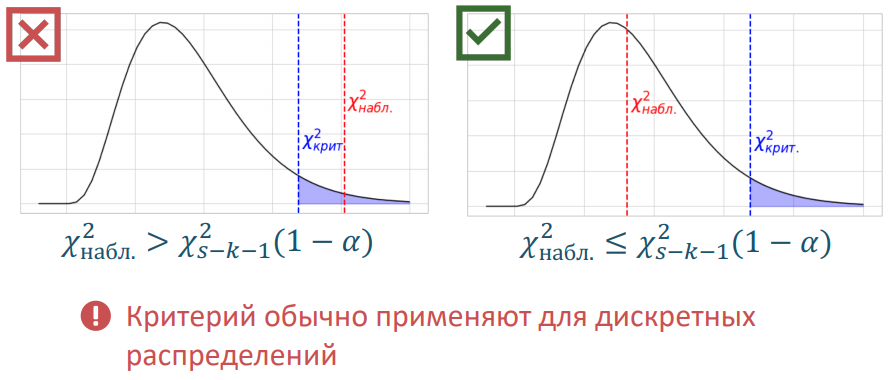
\includegraphics[width=0.3\textwidth]{Screenshot from 2021-09-10 12-03-20.png}

\textit{\textbf{Замечание:}}
\textit{
\begin{itemize}
    \item Критерий Пирсона не состоятелен против всех
альтернатив, т.е. бывают распределения, которые
он не может отличить друг от друга
    \item Можно попробовать использовать критерий
Пирсона для непрерывных распределений
    \item Для этого нужно будет разбить все возможные
значения непрерывной случайной величины
на бины (как на гистограмме) 
    \item Результат работы теста будет зависеть от числа выбранных
бинов $\Rightarrow$ лучше пользоваться для непрерывных
распределений другими критериями
\end{itemize}
}
\textbf{Гипотезы об однородности выборок}\\
Критерий Пирсона по аналогии с критерием Колмогорова
можно использовать для проверки
гипотез об однородности выборок\\
$X_1, ... , X_{n_x} \sim iid F_X(x) \,\, Y_1, ..., Y_{n_y} \sim iid F_Y(x)$\\
$H_0: F_X(x) = F_Y(x)$\\
$H_a: F_X(x) \neq F_Y(x)$\\
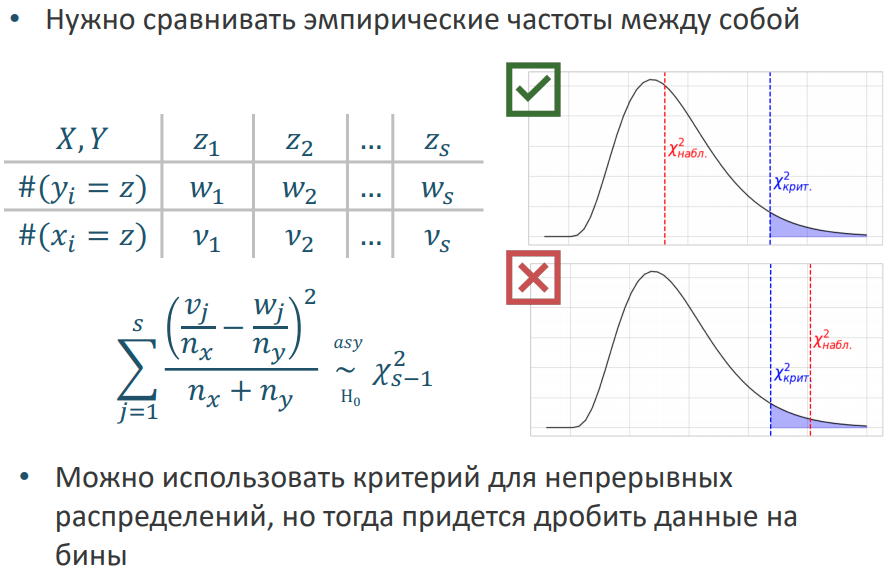
\includegraphics[width=0.3\textwidth]{Screenshot from 2021-09-10 12-12-56.png}

\textit{\textbf{Замечание:}}
\textit{
\begin{itemize}
    \item Его можно использовать и для непрерывных величин, но
результат будет зависеть от числа выбранных групп
\end{itemize}}

\newpage
\section{A/B тесты}
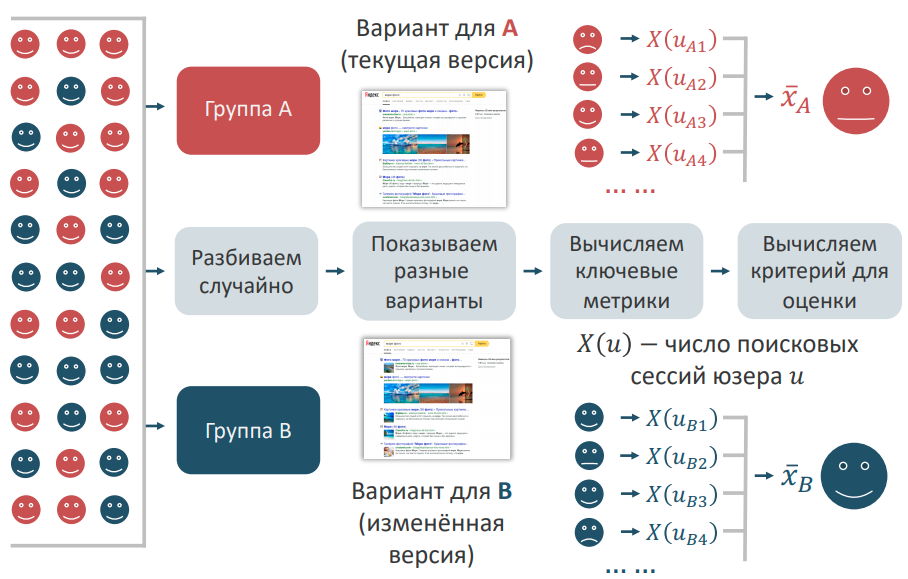
\includegraphics[width=0.3\textwidth]{Screenshot from 2021-09-13 09-54-38.png}
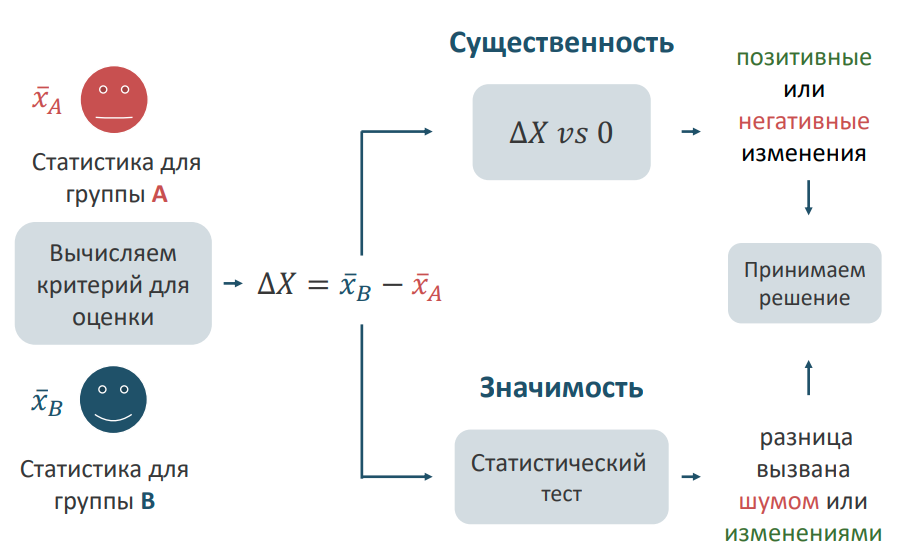
\includegraphics[width=0.3\textwidth]{Screenshot from 2021-09-13 09-57-32.png}
\textbf{Типичные метрики:}
\begin{itemize}
    \item Уникальные пользователи за сессию
    \item Клики на пользователя, клики на один запрос
    \item Среднее время пользователя на сайте
    \item Возвращаемость пользователя
    \item Средний чек
    \item Средний трафик
    \item Средняя разница между ценой товара
            и его себестоимостью (маржа)
\end{itemize}
\textbf{Значимость} – статистический тест говорит нам, что
изменения в метрике неслучайны.\\
\textbf{Существенность} – насколько изменения большие по своей
величине, насколько большой размер эффекта (изменение
метрики), который мы ловим.\\
\textit{\textbf{Замечание:}}\\
\textit{
АБ-тест используется для проверки идей на группе
пользователей. При проведении АБ-теста мы должны
ответить на ряд вопросов:
\begin{enumerate}
    \item Что является целевой метрикой?
    \item На какое увеличение мы рассчитываем?
    \item Какой критерий мы используем для проверки результата
на статистическую значимость?
    \item Как должен выглядеть дизайн эксперимента,
как разбить пользователей на группы?
    \item Как долго должен идти эксперимент?
\end{enumerate}}
\subsection{Множественная проверка гипотез}
\textbf{Проблема:}
Проверяем две гипотезы:\\
$H_0: \mu_1 = \mu_2 = \mu_3$\\
В таком случае можем ошибиться сразу в двух местах(т.е. в одной или в другой):\\
$P(\text{ошибочно отвергнуть хотябы одну из } H_0) = 
1 - P(\text{не ошибиться ни в одной})  = 1 - (1-\alpha)^2 = 2\alpha - \alpha^2 > \alpha$
Т.е. получается наша ошибка первого рода растет, а в случае $n$ гипотез будет рост $1-(1-\alpha)^n$\\
\textbf{Как можем корректировать?}\\
\textbf{Неравенстов Бонферонни}\\
$P(A+B) \leq P(A) + P(B)$ - т.е. можем просто тестировать каждую гипотезу на уровне $\frac{\alpha}{n}$ чтобы в худшем случае получить общий уровень значимости $\alpha$\\
\textbf{Минусы?}\\
\begin{itemize}
    \item Из-за коррекции уровня значимости возникают проблемы с
мощностью тестов
    \item Чем больше гипотез проверяется, тем ниже шансы
отклонить неверные гипотезы
    \item Более того, из-за презумпции нулевой гипотезы для более
низкого уровня значимости нам нужно собрать большее
число наблюдений, чтобы зафиксировать значимое
отклонение от нулевой гипотезы
\end{itemize}
\textbf{Вывод:} Нужно улучшать метод коррекции\\
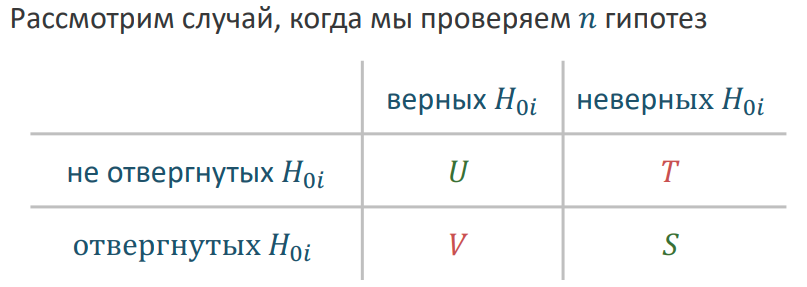
\includegraphics[width=0.3\textwidth]{Screenshot from 2021-09-14 10-27-21.png}
\begin{itemize}
    \item Неверно отклонили $V$ гипотез, неверно не отклонили $T$
гипотез
    \item На практике пытаются контролировать обобщения
ошибки первого рода, например: FWER и FDR
\end{itemize}
\textbf{Групповая вероятность ошибки, FWER (Family-Wise Error Rate)}
– это вероятность совершить хотя бы одну ошибку первого
рода $FWER = P(V>0)$\\
\textbf{Ожидаемая доля ложны отклонения, FDR (False Discovery
Rate) }– это математическое ожидание числа ошибок первого
рода к общему числу отклонений нулевой гипотезы $FDR = E(\frac{V}{V+S})$\\
Т.е. FWER пытается контролировать ошибку первого рода, когда отрицаем верную гипотезу, а FDR пытается контролировать обобщение ошибки второго рода
\subsection{Метод Холма}
\begin{itemize}
    \item Поправка Бонферрони пытается контролировать
FWER (вероятность хотя бы одной ошибки 1 рода)
    \item Метод Холма – улучшение поправки Бонферрони,
обладает более высокой мощностью 
    \item Отсортируем гипотезы по получившимся P-значениям по возрастанию: $p_{(1)} \leq p_{(2)} \leq ... \leq p_{(k)}$
    \item Возьмём для них: $\alpha_{(1)} = \frac{\alpha}{k}, \alpha_{(2)} = \frac{\alpha}{k-1}, ..., \alpha_{(i)} = \frac{\alpha}{k-i+1}, ..., \alpha_{(k)} = \alpha$
    \item Если $p_{(1)} \geq \alpha_{(1)}$ , все нулевые гипотезы не отвергаются, иначе отвергаем первую и продолжаем
    \item Если $p_{(2)} \geq \alpha_{(2)}$ , все оставшиеся нулевые гипотезы не отвергаются, иначе отвергаем вторую и продолжаем
    \item Идём, пока не кончатся гипотезы
    \item Метод Холма обеспечивает контроль FWER на уровне $\alpha$
    \item Метод Холма оказывается мощнее корректировки
Бонферрони, так как его уровни значимости меньше
\end{itemize}
\subsection{Метод Бенджамини-Хохберга}
\begin{itemize}
    \item Отсортируем гипотезы по получившимся P-значениям по возрастанию: $p_{(1)} \leq p_{(2)} \leq ... \leq p_{(k)}$
    \item Возьмём для них: $\alpha_{(1)} = \frac{\alpha}{k}, \alpha_{(2)} = \frac{2\alpha}{k}, ..., \alpha_{(i)} = \frac{i\alpha}{k}, ..., \alpha_{(k)} = \alpha$
    \item Если $p_{(k)} \leq \alpha_{(k)}$ , отвергнуть все гипотезы, иначе не отвергнуть k - ую и продолжить
    \item Если $p_{(k-1)} \leq \alpha_{(k-1)}$ , отвергнуть все гипотезы, иначе не отвергнуть (k-1) - ую и продолжить
    \item Идём, пока не кончатся гипотезы
    \item Для любой процедуры множественного тестирования
    гипотез FDR $\leq$ FWER
    \item Метод Бенджамини-Хохберга обычно оказывается более мощным, чем методы контролирующие FWER
    \item Он отвергает не меньше гипотез с теми же $\alpha_i$
    \item Это происходит за счёт того, что метод позволяет
    допустить большее число ошибок первого рода
\end{itemize}
\subsection{А сколько наблюдений нужно?}
\begin{itemize}
    \item Необходимое количество наблюдений зависит
от размеров ошибок первого и второго рода, а также
от размера эффекта
\item Фиксируем уровень значимости (ошибку 1 рода),
на которую мы согласны
\item Подбираем соотношение между минимальным размером
эффекта, желаемой мощностью и объёмом выборки
\item В выборе соотношении помогает заказчик эксперимента,
у него обычно есть ограничения, с которыми нам придётся
работать (количество магазинов, длительность АБ-теста
и т.п.)
\end{itemize}
\newpage
\textbf{Таблица эффекта-ошибки}
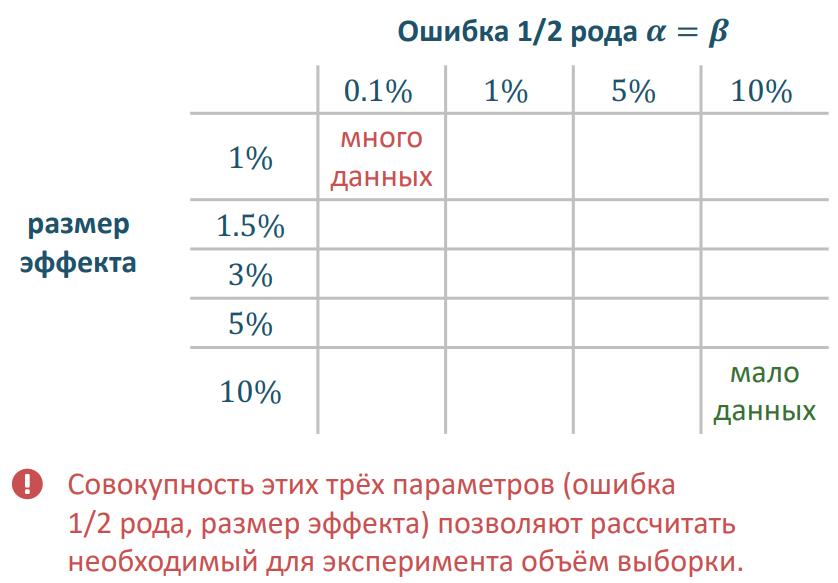
\includegraphics[width=0.3\textwidth]{Screenshot from 2021-09-14 10-51-35.png}
\textbf{Анализ мощности}\\
\textbf{До эксперимента:}
\begin{itemize}
    \item Какой нужен объём выборки, чтобы найти различия
с разумной степенью уверенности
    \item Различия какой величины мы можем найти, если
известен объём выборки
\end{itemize}
\textbf{После эксперимента:}
\begin{itemize}
    \item смогли бы мы найти различия с помощью нашего
эксперимента, если бы величина эффекта была равна $\Delta$
\end{itemize}
\subsection{Метрики для A/B тестирования}
\begin{itemize}
    \item Показатель для улучшения – метрика
\item Метрики бывают разными, они конструируются
в зависимости от бизнес-задачи
\item Иногда метрики привязаны к деньгам
\item Чаще всего денежные метрики грубые (слабо
реагируют на изменения либо, надо очень много
времени, чтобы их измерить)
\item Из-за этого чистым денежным метрикам предпочтительнее
промежуточные метрики
\end{itemize}
\textbf{Роли метрик}
\begin{itemize}
    \item \textbf{Ключевые метрики} – отражают ключевые цели сервиса,
должны обладать безусловной направленностью (если
метрика растёт, сервису всегда становится лучше/хуже)
\item \textbf{Основные критерии оценки изменений} – должны
быть согласованы с ключевыми метриками, должны быть
чувствительными
\item \textbf{Ограничительные метрики} – должны быть чувствительны и
согласованы с тем, что нельзя ломать
\item \textbf{Целевые метрики эксперимента} – должны выбираться
в зависимости от смысла эксперимента
\end{itemize}
$\text{    }\;\;$\\
\textbf{Желательные свойства метрик}
\begin{itemize}
    \item \textbf{Согласованность} – метрика должна быть согласована
с целями сервиса и его ключевыми метриками
\item \textbf{Направленность} – если значение метрики изменилась,
должна быть чёткая интерпретация этого изменения
(хорошо это или плохо)
\item \textbf{Чувствительность (sensitivity) }– способность метрики
отражать статистически значимую разницу между
контрольной и тестовой группами, когда она есть. Чем выше чувствительность, тем меньше данных нужно,
чтобы обнаружить статистически-значимые изменения.\\
\textbf{Пример:} метрики, основанные на деньгах слабо
реагируют на изменения
\item \textbf{Стабильность} – метрика должна быть чувствительной
и согласованной с тем, что нельзя ломать. Если у метрики высокая дисперсия, то для того, чтобы
уловить значимый эффект, надо собирать много данных\\
\textbf{Пример:} розничный торговый оборот магазина
может колебаться в очень широких диапазонах.
Чтобы уменьшить его дисперсию, обычно смотрят
торговый оборот отдельных отделов.
\item 
\end{itemize}
\textbf{Примеры:}\\
\textbf{Лояльность пользователя:}
\begin{itemize}
    \item Число пользовательских
сессий
    \item Время, которое юзер
проводит в сервисе
\end{itemize}
Имеют чёткую направленность\\
Хорошие предикторы для долгосрочного успеха
продукта\\
Обладают слабой чувствительностью\\
\textbf{Активность пользователя:}
\begin{itemize}
    \item Число кликов за сессию
    \item Длина пользовательской
сессии
\end{itemize}
Обладают сильной чувствительностью\\
Обладают неоднозначной направленностью\\
\textbf{Пример:} клики пользователей в рекомендательной системе
отражают как позитивные, так и негативные сигналы
\begin{itemize}
    \item С одной стороны, они говорят, что пользователю
нравится пользоваться продуктом
\item С другой, они говорят, что у нас много
кликбейтного контента
\item Метрики с чёткой интерпретацией часто обладают низкой
чувствительностью
\end{itemize}

% \newpage
\end{multicols}

\end{document}
